\subsection{Partial differential equations}\label{sec:PDE}
A differential equation is an expression of a function in terms of it's derivative(s), in such a way that the function itself can be determined through solving the equation \citep[p. 1-4]{tveitoPDE}. I.e. the solution to a differential equation will be the function that satisfies the equation. Differential equations are again split into two main categories, \textit{ordinary differential equations} (ODE) and \textit{partial differential equations} (PDE). An ODE involves only derivatives with regards to a single variable, while PDEs include the partial derivatives of a multi-variable function. This report will only cover PDEs. 

\begin{equation}
\label{eq:gen_pde}
    (\mathcal{L}u)(x) = f(x), \quad x\in \Omega
\end{equation}

The most general PDE form is often written as Eq. \ref{eq:gen_pde}.
In this representation, $\Omega \subset \mathbb{R}^d$ is the domain, $f: \mathbb{R}^d \to \mathbb{R}$ is a (continuous) function, and $u: \mathbb{R}^d \to \mathbb{R}$ is the unknown function.
$\mathcal{L}$ is a given differential operator.
In general, $\mathcal{L}$ can contain any combination of partial derivatives of $u$, however most popular PDEs are limited to linear combinations of partial derivatives.
An example of a possible differential operator is $\mathcal{L}u = \frac{\partial^2 u}{\partial t^2} - c^2 \frac{\partial^2 u}{\partial x^2}$, which, if $f(x) = 0$, leads to the one-dimensional wave equation.

% Here $u$ denotes some multi-variable function with variables $\bold{x}$, where $x_i$ and $x_j$ denote two of these variables. Furthermore $\frac{\partial u(\bold{x})}{\partial x_i}$ denotes the partial derivative of the function with regards to the $i$-th variable. $K(\bold{x})$ is some other function of the variables. The degree of derivation is arbitrarily chosen for the examples above, and may vary in either direction for different equations. Very commonly PDEs will more specifically regard a time-dependent function $u(\bold{x}, t)$. This is especially common for any PDE modelling real-world systems. 

The solution of a PDE can normally be found either analytically by solving the equation directly, or through a broad range of numerical methods. These methods usually provide an approximation of the exact solution, but by tweaking parameters the approximate solution will commonly converge towards the exact. Numerical approximations will be further covered in section \ref{sec:FD}.

\subsubsection{Initial and boundary conditions}
Solving a PDE from only an equation as given above will provide a general solution, often involving non-determinable constant terms or coefficients. To further solve for these and find unique solutions, one requires \textit{initial conditions} or \textit{boundary conditions}. For a problem including such conditions, a solution is only valid when satisfying both the equation and additional conditions. 

Initial conditions are normally associated with time-dependent systems, but can be generalized to other dimensions. Such conditions describe the state of a system at the "beginning" of the relevant dimension. For a time-dependent system the condition will then be for $t=0$. 
% Initial conditions for time-dependent systems are commonly given on the form: 
% \begin{equation}
%     u(\bold{x}, 0) = g(\bold{x})
% \end{equation}
% $g$ represents a general expression and can be a scalar, a function, or a vector - depending on the nature of the problem. 

Boundary conditions are similar to initial conditions, but instead of describing a state at some starting point the condition now provides the state of the system at some boundary point. These points describe the states at the edges of a functions domain. 
% For a PDE of a function $u(x,t)$ on the domain $[0, L]$, the boundary conditions might be stated
% \begin{equation}
%     \begin{split}
%         u(0, t) &= g_1(t), \quad t\geq0 \\
%         u(L, t) &= g_2(t), \quad t\geq0
%     \end{split}
% \end{equation}


\subsection{Diffusion equation}\label{sec:diffeq}
\textit{The diffusion equation} is one of the most commonly encountered PDEs, and describes the spread of particles through matter over time \citep[p. 18]{tveitoPDE}. For one dimension, and uniform materials, the general equation is given as:
\begin{equation}
    \frac{\partial u(x,t)}{\partial t} = D \frac{\partial^2 u(x,t)}{\partial x^2}
\end{equation}
Here $D$ is a constant indicating the rate of the diffusion, called the diffusion coefficient. 

Arguably the most famous among variations of the diffusion equation is one obtained where $D=1$, commonly known as the heat equation:
\begin{equation}\label{eq:diffu}
    \frac{\partial u(x,t)}{\partial t}=\frac{\partial^2 u(x,t)}{\partial x^2} , \ t>0, \ x\in [0, L]
\end{equation}
The heat equation (and similarly other PDEs) is also commonly denoted in a short-hand version where the partial derivatives are stated in subscript of $u$:  
\begin{equation}\label{u_tu_xx}
    u_t = u_{xx}
\end{equation}
$\frac{\partial u(x,t)}{\partial t}$ is denoted $u_t$ and $\frac{\partial^2 u(x,t)}{\partial x^2}$ is denoted $u_{xx}$.

One way to interpret the equation is to think of the dispersion of heat through a uniform rod of length $L$. Given some initial state of temperatures in the rod, the equation describes how the heat then diffuses through the rod over time. 

Initial conditions for the heat equation are given on the form: 
\begin{equation}\label{init_cond}
    u(x,0) = f(x),
\end{equation}
where $f(x)$ is a function describing how the heat is disbursed through the rod at $t=0$.
Similarly boundary conditions are given on the form: 
\begin{equation}\label{bound_cond}
    \begin{split}
        u(0, t) = g(x), \quad t \ge 0 \\
        u(L, t) = h(x), \quad t \ge 0
    \end{split}
\end{equation}
The functions $g$ and $h$, describe how the temperature changes over at time at the ends of the rod (the boundary points). 
$f, g, h$ from Eq. \ref{init_cond} and Eq. \ref{bound_cond}, can either be functions varying by x or constants, depending on the system described by the PDE. 
Normally the functions will evaluate to a scalar, resulting in the following conditions: 
\begin{equation}
    \begin{split}
        u(0, t) = \alpha, \quad t\geq0 \\
        u(L, t) = \beta, \quad t\geq0
    \end{split}
\end{equation}

\subsubsection{Analytical solution}\label{sec:anal_sol}
This report considers the heat equation with $L=1$, the initial condition
\begin{equation}
u(x, 0) = \sin(\pi x)    
\end{equation}
and boundary conditions
\begin{equation}
    u(0, t)=0 \quad t\ge0
\end{equation}
\begin{equation}
    u(L, t)=0 \quad t\ge 0.
\end{equation}

For this given equation, with conditions above, the analytical solution is found to be: 

\begin{equation}\label{analytical_sol}
    u(x,t) = \sin(\pi x) e^{-\pi^2 t}
\end{equation}

By insertion in the PDE and it's conditions this is easily verified. The full derivation by separation of variables, as well as verification of the solution, can be found in Appendix \ref{appendixB}.

\subsection{Finite difference schemes}\label{sec:FD}
While the analytical solution is relatively simple to find for some PDEs, such as the diffusion equation shown above, other PDEs are difficult or impossible to solve analytically.
When considering these PDEs, we usually find an approximation to the solution.
There are many ways of doing this, including collocation methods, Galerkin methods, finite element methods, and finite difference schemes.
Due to them being easy to implement, flexible, and theoretically approachable, finite difference schemes are very popular \citep[p. 119]{tveitoPDE}.

The main idea behind finite difference schemes is to divide your domain into discrete points.
Given a PDE $\mathcal{L}u=f$, $u : [0, L] \times [0, T] \to \mathbb{R}$, we start by creating discrete points $(x_j, t_n) = (j \Delta x, n\Delta t)$, where $\Delta x = L/N_x$ and $\Delta t = T/N_t$.
We denote the approximation at each point by $u_j^n = u(x_j, t_n)$.

We proceed by approximating the derivatives of the PDE using Taylor expansions around $u_j^n$.
\begin{align}
    \label{eq:fd_dt}
    \frac{\partial u}{\partial t}(x_j, t_n) &= \frac{u_j^{n+1}-u_j^n}{\Delta t} \\
    \label{eq:fd_dx2}
    \frac{\partial^2 u}{\partial x^2}(x_j, t_n) &= \frac{u_{j+1}^n - 2u_j^n + u_{j-1}^n}{\Delta x^2}
\end{align}

In the diffusion equation introduced in section \ref{sec:diffeq}, we approximate the two partial differentiation terms as described in Eq. \ref{eq:fd_dt} and Eq. \ref{eq:fd_dx2}.
The approximation in Eq. \ref{eq:fd_dt} has error term of order $\mathcal{O}(\Delta t)$, while Eq. \ref{eq:fd_dx2} has error term of order $\mathcal{O}(\Delta x^2)$.
The derivation of both approximations from Taylor expansions of the function $u(x, t)$ around $(x_j, t_n)$ are included in Appendix \ref{appendixC}.

\begin{equation}
    \label{eq:diff_scheme}
    \frac{u_j^{n+1}-u_j^n}{\Delta t} = \frac{u_{j+1}^n - 2u_j^n + u_{j-1}^n}{\Delta x^2}
\end{equation}

Equation \ref{eq:diff_scheme} describes the entire finite difference scheme for the PDE defined in Eq. \ref{eq:diffu}.
This scheme is a forward Euler scheme, as the approximations of the time derivative between $t_n$ and $t_{n+1}$ are made using values at time $t_n$ on the right side of equation $\ref{eq:diff_scheme}$.
The schemes "step" through time, by solving Eq. \ref{eq:diff_scheme} with respect to $u_j^{n+1}$.
\begin{figure}[h]
        \centering
        \begin{tikzpicture}
            \stencilpt{-1,0}{i-1}{$u_{j-1}^n$}{below};
            \stencilpt{ 0,0}{i}  {$u_{j}^n$}{below};
            \stencilpt{ 1,0}{i+1}{$u_{j+1}^n$}{below};
            \stencilpt{ 0,1}{n+1}{$u_{j}^{n+1}$}{right};
            \draw
            (i-1) -- (i)
            (i)   -- (i+1)
            (i) -- (n+1);
            
            % \node[fit=(i-1)(i+1)(n+1), draw=black, inner xsep=6pt, inner ysep=12pt] {};
        \end{tikzpicture}
        
        \caption{The stencil of the scheme defined by Eq. \ref{eq:diff_scheme}.} 
        \label{fig:fd_stencil}  
    \end{figure}
The scheme can be viewed as a stencil, as shown in Fig. \ref{fig:fd_stencil}, where the values at time $t_n$ are known and used to calculate the values at time $t_{n+1}$.
Note that all values at time $t_0$ are known from the initial condition.
\subsubsection{Stability}
Considering the stability of the approximation obtained from the scheme, is important when using finite difference schemes to solve PDEs.
Using a very small value of $\Delta x$ compared to $\Delta t$, leads to the second derivative of $x$ at the right side of equation \eqref{eq:diff_scheme} being very accurate for a small area of the function, while the time step it is used for is really big.
This could cause large error, and we might end up with large oscillations that do not match the analytical solution.
\begin{equation}
    \label{eq:stability}
    \frac{\Delta t}{\Delta x^2} \leq \frac{1}{2}
\end{equation}
Equation \eqref{eq:stability} is the stability requirement of the scheme defined by equation \eqref{eq:diff_scheme} \citep[p. 130]{tveitoPDE}.
A derivation of this is also included in Appendix \ref{appendixD}.

\subsection{Neural Networks} \label{sec:NN}
\textit{Parts of this subsection is reused from our previous work \citep[p. 7-10]{project2}.}

% Although methods like linear regression for continuous tasks and logistic regression for classification are suitable for a lot of applications, a more adaptive and versatile method is necessary to broaden the possibilities of use. 
As an alternative to finding solutions analytically or using numerical approximation methods, which are specialized for the task, it has become widely popular in recent years to utilize \textit{neural networks} to solve PDE's.

% \textit{Neural networks} (NN) make no assumptions about underlying data-structures, and can be fit for a broad range of tasks, including regression and classification \citep[Neural networks]{morten}. Through \textit{layers} of \textit{nodes} (often called \textit{units}), the network imitates the process of neurons firing in the brain, and can be fit to many complex problems.

\begin{figure}[H]
    \centering
    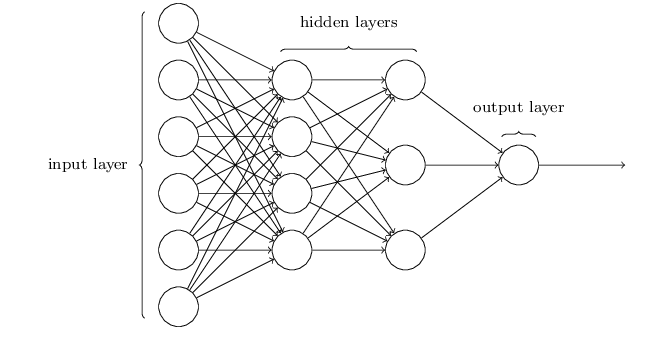
\includegraphics[width=1\linewidth]{project_2/figures/generic_NN.png}
    \caption{Illustration of a generic neural network. \cite[Taken from][Ch.1]{nielsen}.}
    \label{fig:NN}
\end{figure}

A general NN consists of an input layer, $k$ hidden layers and an output layer - all consisting of a varying number of nodes or units, as visualized in Fig. \ref{fig:NN}. The number of nodes in a layer is denoted as the width of the layer, and the number of layers in a network is denoted the depth of the network. 
Hidden layers are not hidden in the sense that they're not a visible part of the model; but rather that when using a trained model one never interacts with anything past the input and output layers, thus the internal nodes appear as hidden. 
Between the nodes we have connections called \textit{weights}. These determine the influence from one particular node to another. 

The weighted model stems from the mathematical function for an artificial neuron given as follows; 

\begin{equation}\label{artifical_neuron}
    y = f\left( \sum_{i=0}^Nwx_i \right) 
\end{equation}

Here $f$ is some \textit{activation function} that takes a weighted sum of $N$ inputs and maps them to an output. Activation functions are further covered in the next subsection, \ref{sec:activation_func}.

How many layers an NN has, how many nodes each layer has and how they're connected make up what's called the \textit{architecture} of the neural network \citep[Ch.1]{nielsen}. These decisions are normally made case-by-case depending on the task at hand, input size, desired output size, etc. Apart from compatible dimensions there are no clear choices for what constitutes a "better" architecture, however more complex tasks are commonly better solved by more "complex" networks; i.e. more layers and more nodes. 

The simplest model for an artificial neural network is called a \textit{feed forward neural network} (FFNN), where logically enough the flow of information moves only in one direction; forward. Consider for instance a FFNN with one hidden layer. The input-layer receives the input $X$, which is then passed through the first weights $W_0$ to the second layer. Here the weighted sum is passed through an activation function $f_1$ and passed via $W_1$ to the output layer. In the output layer the weighted sum is passed through $f_2$, before finally being output from the model. 
For each node $n$ the process can be formally expressed as:


\begin{equation}
    y = f\left( \sum_{i=0}^N w_{0n}x_i + b\right)
\end{equation}
\citep[p.17]{Ketkar2017}. Here one can clearly see the similarities to Eq. \ref{artifical_neuron}. $b$ represents what is called a \textit{bias term}. Looking back to the structural similarities of a biological NN, the bias allows one to skew "how easy it is to get the neurons to fire". I.e., by altering the bias terms one can shift the the output values in a desired direction - in theory. This is however easier said than done, and altering either weights or biases directly is not common procedure. Instead one relies on a good choice of cost function and the training of the NN to produce fitting parameters. 


\subsubsection{Activation functions}\label{sec:activation_func}

The activation functions are the key to the complexity that allows NNs generalize to so many different tasks. For an NN with one hidden layer and activation functions given as:
\begin{align}
\begin{split}
    f_1(\bold{x})&=\bold{W_0}^T\bold{x} + b_1 \\
    f_2(\bold{x})&=\bold{W_1}^T\bold{x} + b_2 
\end{split}
\end{align}
The entire network could then be expressed: 
\begin{align}\label{linear_nn}
    \begin{split}
        F(\bold{x})&=f_2(f_1(\bold{x})) \\
        &= \bold{W_1}^T(\bold{W_0}^T\bold{x} + b_1) + b_2 \\
        &= \bold{W_1}^T\bold{W_0}^T\bold{x}+\bold{W_1}b_1+b_2 \\
        &=\bold{W}^T\bold{x}+b
    \end{split}
\end{align}
In other words, the entire NN itself is just one big chain of all it's weights and activation functions nested. Were the activation functions to be linear the network itself would be linear, as shown in the example above \citep[p.168]{Goodfellow-et-al-2016}. This undermines the fundamental purpose of using an NN, as it's generally favorable with simpler models for linear problems. 

Beyond non-linearity there are few hard restrictions on the activation functions, granted some are to be preferred.
The rest of this section will use the convention of $\bold{z}$ representing the vector of "raw output" from the previous layer. Raw output simply refers to the values before they're passed through the activation function. An activation function applied to the entire vector, is simply applied element-wise - i.e. the input and output are congruent and
\begin{equation}
    f(\bold{z})_i = f(z_i)
\end{equation}

One example of a common activation function is the Sigmoid function \citep[Logistic Regression]{morten}: 
\begin{equation}\label{sigmoid}
    f(\bold{z})_i=\sigma(z_i)=\frac{1}{1+\exp(-z_i)}=\frac{\exp(z_i)}{1+\exp(z_i)}
\end{equation}
$\sigma$ takes in any number on the real number-line, and maps it to the interval $(0,1)$. The Sigmoid is normally used for internal nodes or classification tasks. 
% Alternatively the \textit{softmax} function is another common function for classification \citep[Logistic Regression]{morten}. 
% This is an extension of the Sigmoid function, and is also what's used in place of the sigmoid function for multinomial linear regression.
% The softmax function normalizes a vector of input values so that the resulting outputs sum to $1$. While softmax can be used in internal nodes, it is more commonly used for the output layer. For an input vector of size $K$ the softmax function for each element i is given as: 
% \begin{equation}\label{softmax}
% f(\mathbf{z})_i = \frac{e^{z_i}}{\sum_{j=1}^K e^{z_j}}
% \end{equation}

Another common choice is the activation function \textit{Rectified Linear Unit} (ReLU) \citep[Building a feed forward neural network]{morten}; 
\begin{equation}\label{relu}
    f(\bold{z})_i=\max\{0, z_i\}
\end{equation}
Alternatively expressed as
\begin{equation}
    f(\bold{z})_i = \begin{cases} 
      z_i & \text{if } z_i > 0 \\
      0 & \text{if } z_i \leq 0 
   \end{cases}    
\end{equation}
As opposed to the sigmoid function, ReLU does not \textit{saturate} for large positive values. The saturation of a function is an issue where the values of the function approaches its maximum or minimum, resulting in vanishing gradients and thereby poor convergence. However, ReLU suffers from an issue called \textit{the dying ReLU}. In essence this refers to nodes stagnating at zero; effectively dying. 

One solution to the problem of the dying ReLU is to use \textit{leaky ReLU} \citep[p. 190]{Goodfellow-et-al-2016}; 
\begin{equation}
    f(\bold{z})_i=\max\{0, z_i\}+\alpha\min\{0,z_i\}
\end{equation}
Here $\alpha$ is typically sat to a small value, like $0.01$. 
Similiar to ReLU, Leaky ReLU can alternatively be expressed as; 
\begin{equation}
    f(\bold{z})_i = \begin{cases} 
      z_i & \text{if } z_i > 0 \\
      \alpha z_i & \text{if } z_i \leq 0 
   \end{cases}
\end{equation}
This variation of ReLU allows for some portion of the negative values to be included, mitigating the risk of dying nodes. 
% Examples: sigmoid, ReLU, leaky ReLU, softmax, identity in last layer?

A fourth choice, and arguably the most popular one for deep neural networks, is the \textit{tanh} function - also known as the hyperbolic tangent function \citep[Neural Networks]{morten};
\begin{equation}
    f(\bold{z})_i = \tanh(z_i)=\frac{e^{z_i}-e^{-z_i}}{e^{z_i}+e^{-z_i}}
\end{equation}
As tanh is symmetrical, mapping to both negative and positive values, it is less prone to saturation than the sigmoid - however it still might be an issue. 

The output layer of a NN will often have a different activation function than it's predecessors. While the choice of activation functions in the hidden layers have less direct consequences to the type of output, the last activation dictates exactly this.
% For classification tasks one often has either the sigmoid or similar functions for the output layer. 
Commonly less restrictive functions are used for regression problems than classification problems, to avoid limiting the possible output scope of the network. Some even choose to use the identity function, or similarly no activation function, for the last layer:
\begin{equation}
    f(\bold{z})_i=z_i
\end{equation}

\subsubsection{Initialization of weights and biases}\label{sec:NN_init}

To start training the NN, and navigating the landscape of the cost function, one needs a starting point \citep[p.297]{Goodfellow-et-al-2016}. For initialization of weights and biases there are a lot of different conventions. How the values are initialized can affect things like the optimization itself, convergence and the generalization of the model. 
One of the most important aspects is to ensure that no nodes are the same; for nodes with the same activation function, same input values and same initial values, most training methods will update these in the same manner. This again will result in a more narrow search field were not all possibilities in the cost landscape can be reached. Although there exists ways to work around this problem, it is commonly preferred to avoid this issue altogether as best one can. 
Larger (distinct) initial weights will be more effective against symmetry, but will on the other hand heighten the risk of problems like exploding gradients and saturated nodes. 

Arguably the most common method across the field, is random initialization. As the wording entails, the weights and biases are then randomly initialized. The randomness method alleviates the chances of symmetrical nodes, while the distribution chosen can help mitigating the risk of too large weights. The values are often selected from a Gaussian distribution, with mean zero and standard deviation 1. 

% https://cs231n.github.io/neural-networks-2/
% Among more specialized methods we find the methods called \textit{Xavier Glorot} \cite{Glorot} and \textit{Kaiming He} \cite{He}, normally denoted just Glorot and He. These are both variations of random initialization, but are furthermore motivated in ensuring that the variance of input to one layer and output to next is the same. By doing so one prevents the variances from growing or shrinking exponentially as they propagate through the layers, which can lead to exploding or vanishing gradients. In modern machine learning, these are the two most widely used methods.
% \begin{equation}\label{glorot}
%     W_{i,j} \sim U\left(-\sqrt{\frac{6}{m+n}},{\sqrt{\frac{6}{m+n}}},\right)
% \end{equation}
% \begin{equation}\label{he}
%     W_{i,j} \sim \mathcal{N}\left(0, \frac{2}{\sqrt{n}}\right)
% \end{equation}
% Eq. \ref{glorot} shows the normalized uniform distribution from which the weights are selected in Glorot, and Eq. \ref{he} the normalized normal distribution from which values are selected in He. In both equations $W_{i,j}$ denote the weights between the $i$-th and $j$-th layers, and $m$ and $n$ the size of the $i$-th and $j$-th layer respectively. Although the methods were proposed as given above in their respective papers, it is not uncommon to implement Glorot as a normal distribution, and He as a uniform distribution. As of now there exists no common consensus of which versions are better, neither theoretically or empirically, and thus the choice is for each specific case.

% Glorot is derived specifically for the Sigmoid function, and He for the ReLu function. It often yields faster convergence, and sometimes better performance, using the accompanying initialization methods for networks using the aforementioned activation functions. 

Among more specialized methods we find the methods called \textit{Xavier Glorot} \cite{Glorot} commonly denoted just Xavier or Glorot. This is a variation of random initialization, but is furthermore motivated in ensuring that the variance of input to one layer and output to next is the same. By doing so one prevents the variances from growing or shrinking exponentially as they propagate through the layers, which can lead to exploding or vanishing gradients. In modern machine learning, this is one of the most widely used methods.
\begin{equation}\label{glorot}
    W_{i,j} \sim U\left(-\sqrt{\frac{6}{m+n}},{\sqrt{\frac{6}{m+n}}},\right)
\end{equation}
Eq. \ref{glorot} shows the normalized uniform distribution from which the weights are selected in Glorot. $W_{i,j}$ denote the weights between the $i$-th and $j$-th layers, and $m$ and $n$ the size of the $i$-th and $j$-th layer respectively. Although the method was proposed as given above in paper piloting this method, it is not uncommon to implement Glorot with a normal distribution. The weights are then drawn from the normalized normal distribution provided as:
\begin{equation}
    W_{i,j} \sim \mathcal{N}\left(0, \frac{2}{\sqrt{m+n}}\right).
\end{equation}
As of now there exists no common consensus of which version is better, neither theoretically or empirically, and thus the choice is left for each specific case.

Glorot is derived specifically for the Sigmoid function, but performs well on other activation functions as well. Especially when accompanying the Sigmoid function, it often yields faster convergence, and sometimes better performance.

\subsubsection{Choice of cost function for neural networks}
In addition to initialization of weights and biases, the training of the model largely depends on choice of cost function, which again depends on the task at hand. How a cost function looks has in itself no restrictions, but some are more suited than others.
The choice of cost function is arbitrarily what dictates the landscape that is navigated in the optimization of a network. Most popular optimization techniques require a cost function that can be expressed in terms of a loss function, i.e. that can be computed for each data point on its own. 
For networks to be used on regression problems one commonly uses \textit{Mean Squared Error} (MSE), given as: 
\begin{equation}\label{mse}
    \text{MSE} = \frac{1}{n}\sum_{i=0}^{n-1}(y_i-\Tilde{y}_i)^2.
\end{equation}

\subsubsection{Training the network}
For the actual training of the network, in other words finding the optimal weights and biases, one normally uses gradient descent (see section \ref{sec:gd}). The first step in this process is finding the gradients of the cost function to navigate the parameter landscape. As each layer of a NN can be expressed as a function of its previous layer, one can imagine these expressions to quickly become quite complicated. Furthermore we have to find the partial derivatives for all weights and biases. The most used solution to this intricate problem, is called \textit{backpropagation} \citep[p. 200]{Goodfellow-et-al-2016}. While many libraries provide implementations of automatic gradients, such as PyTorch's Autograd \cite{Ansel_PyTorch_2_Faster_2024} and Tensorflow's GradiantTape \cite{Abadi_TensorFlow_Large-scale_machine_2015}, it is beneficial to understand how manual backpropagation works. Not only is this useful for debugging and ensuring code behaves as expected, but it is essential for understanding the training process. 

The fundamental concept of backpropagation is the use of the chain rule from calculus. Since the network's output is a composition of functions, the chain rule allows us to systematically propagate backwards through the network and compute the derivatives effectively \citep[Ch.2]{nielsen}. 

Denoting the output of layer $(l)$ as $ a^{(l)}$ and the weights and biases for that layer as $W^{(l)}$ and $b^{(l)}$, respectively. For a given layer, the input $z^{(l)}$ to the activation function is:

\begin{equation}
z^{(l)} = W^{(l)} a^{(l-1)} + b^{(l)}
\end{equation}

Here $a^{(l-1)}$ is the output (or activation) from the previous layer. The activation \( a^{(l)} \) is then given by applying the activation function $f$ to $z^{(l)}$:

\begin{equation}
a^{(l)} = f(z^{(l)})
\end{equation}

To calculate how each weight $ W^{(l)}$ and bias $b^{(l)}$ affects the overall cost $L$, we start from the final layer and compute the gradient of the cost with respect to each parameter in the network, working backward through each layer. The gradient of the cost with respect to $W^{(l)}$ is obtained using the chain rule:

\begin{equation}
\frac{\partial L}{\partial W^{(l)}} = \frac{\partial L}{\partial a^{(l)}} \cdot \frac{\partial a^{(l)}}{\partial z^{(l)}} \cdot \frac{\partial z^{(l)}}{\partial W^{(l)}}
\end{equation}

where:
\begin{itemize}[label=--]
    \item $\frac{\partial L}{\partial a^{(l)}}$ is the gradient of the cost with respect to the layer’s activation
    \item $\frac{\partial a^{(l)}}{\partial z^{(l)}}$ is the derivative of the activation function applied at layer $l$
    \item $\frac{\partial z^{(l)}}{\partial W^{(l)}}$ is the derivative of the weighted sum with respect to the weights.
\end{itemize}

By recursively applying this process from the output layer back to the input layer, back-propagation computes all necessary gradients efficiently, enabling gradient descent to adjust each parameter and reduce the cost.

\subsection{Gradient descent}\label{sec:gd}
\textit{Parts of this subsection is reused from our previous work \citep[p. 4-6]{project2}.}

%morten lecture notes
For complicated methods like neural networks, optimal values for our parameters are seldom straight forward to obtain, and often numerical approximation is the only feasible approach \citep[Week 40]{morten}.  
One method for this type of numeric optimization, and arguably the most popular one, is \textit{gradient descent} (GD). In addition to benefits of efficiency and performance, gradient descent triumphs in it's versatility as it can be used for a wide range of optimization problems - including linear regression, logistic regression, neural networks, and many more. 

Imagining the graph of a cost function as a hilly landscape; global and local minima as valleys, poorer solutions as hills - GD seeks to land in the deepest valley, i.e. the global minimum. 
By looking at the slope of the landscape one can keep taking steps in the steepest descending direction, and this way hopefully end up at the global minimum.

\begin{equation}\label{eq:gd}
    -\nabla_\theta C(\theta) = -\begin{bmatrix}
\frac{\partial C}{\partial \theta_1} \\
\frac{\partial C}{\partial \theta_2} \\
\vdots \\
\frac{\partial C}{\partial \theta_n}
\end{bmatrix}
\end{equation}

More precisely, one finds the gradient of the cost function with respect to the parameters of the model - which provides the direction of steepest increase. The negative of the gradient will then provide the direction of steepest decrease, as given for a general cost function in Eq. \ref{eq:gd}. $\theta$ represent the entire model, while the $\theta_i$s represent each of the parameters present in the model.

\begin{equation}\label{eq:updt_std}
    \theta_{t+1} = \theta_t - \eta_t \nabla_{\theta} C(\theta_t)
\end{equation}

When updating the parameters in the model, we now use this gradient combined with a new parameter $\eta$, as shown in Eq. \ref{eq:updt_std}.
$\eta$ is commonly known as the \textit{learning rate}, which we will discuss further below.

For a model containing only a few data-points and parameters, computing the gradient in each step is feasible.
However, when considering larger models and data sets with more parameters and training points (and complicated numerical processes computing the gradients), standard gradient descent becomes very computationally heavy, and is often avoided.
Commonly it is then replaced by \textit{stochastic gradient descent} (SGD).
% In literature there are two main views on how SGD is motivated, with slight variations for the implementation.
SGD computes approximations of the gradients using subsets of the training data, and thereby reducing computational cost.

% The first approach is presented in \textcite[p. 291]{Goodfellow-et-al-2016}. For each iteration (\textit{epoch}) of the training process one \textit{mini-batch} of size $k$ is randomly chosen. Each epoch a new batch is randomly chosen. 
% The motivation behind this approach is to achieve a good approximation to the gradient in each step, while making each step less computationally heavy.

% An alternative approach can be found in \textcite[p. 47]{raschka}.
In it's purest, theoretical form SGD computes a gradient for a single datapoint at the time - but in practice it is far more common to use mini-batches. The training data is then split into $m$ equal mini-batches in each epoch, and these mini-batches are looped over; calculating the gradients and updating the model for each batch \textcite[p. 47]{raschka}.
Each epoch is about as computationally heavy as in normal gradient descent. However the model parameters are updated more frequently, thus convergence is reached faster and the overall computational complexity is reduced.

% In essence, the two versions are virtually equivalent. Each step in the inner loop of Raschka's version and each epoch in Goodfellow's, are effectively the same. For coinciding values of $k$ and $m$, the batches will even be congruent for each iteration. Raschka's method may converge slightly faster by updating parameters more frequently, while Goodfellow's introduces a slightly higher degree of randomness by choose each batch with replacement. However, as the size of the dataset and number of epochs increases, this difference becomes negligible.
% For the rest of the report, any mention of SGD is to be understood as an implementation by Goodfellow's version.

\subsubsection{Learning rate}
For both GD and SGD, the gradients are multiplied by a \textit{learning rate} $\eta_t$ when updating the model.
This learning rate is a positive scalar, usually chosen of small value to make each update relatively small \citep[p. 84]{Goodfellow-et-al-2016}.
As a gradient is only representative for the change at the exact point of calculation, making too large of an update to the model based on a gradient is risky. By changing the model to much, i.e. moving it too far in the landscape, one could be moving to areas of the function that are topographically very different than the starting point. In the worst case, a large step could overshoot the minimum.

While having too large of a learning rate could result in overshooting the minimum, and hence not reaching convergence; too small of a learning rate also has it's disadvantages. 
The smaller the learning rate, the more iterations are required to approach the minima, causing the training to become computationally heavier. To find a balance between the two, some opt for choosing a learning rate by trial error.
% One might still elect to choose a constant model by trial and error.
% Since the drawbacks of a low learning rate are most unfavorable in the early iterations, and a too high learning rate mostly causes problems in the later iterations, an intuitive solution is to start with a higher learning rate and reduce it after a set number of iterations.
% \begin{equation}\label{eq:line_search}
%     C(\theta_t - \eta \nabla_\theta C(\theta_t))
% \end{equation}
% Another approach is calculating the function in Eq. \ref{eq:line_search} for different values of $\eta$, and choosing the $\eta$ resulting in the smallest value. This technique is called \textit{line search} \citep[p. 84]{Goodfellow-et-al-2016}.
% As computing every possible value of $\eta$ would resemble an exhaustive search, line search still requires us to manually choose a set of learning rates, and every step in the iteration is limited to choose one of those learning rates.
A more common alternative is to opt for \textit{adaptive learning rate} algorithms.

% \subsubsection{Adaptive learning rates}
% Both regular and stochastic gradient descent faces several issues when trying to approach the global minimum.
In addition to constant learning rates being hard to tune, problematic points in the loss function such as local minima and saddle points can cause the iterative procedure to lose progress \citep[p. 116-117]{Ketkar2017}.
To address these issues, a series of algorithmic variations have been proposed to replace the step of updating the model (Eq. \ref{eq:updt_std}).
% A common technique in these algorithms, is to utilize information from the previous updates to improve the next one.
% One of the more simple algorithms achieving this, is the \textit{momentum} algorithm.
% In this algorithm, one uses a fraction of the update from the previous step, to help us guide the next.
% \begin{align}\label{eq:updt_mom}
% \begin{split}
%     v_t &= \gamma v_{t-1} + \eta_t \nabla_{\theta}C(\theta_t) \\
%     \theta_{t+1} &= \theta_t - v_t
% \end{split}
% \end{align}
% Note that this algorithm requires us to tune two constants ($\eta$ and $\gamma$), instead of only one constant as in the original case.
% Other optimizing methods focus on adjusting the learning rate for each iteration. One such algorithm is the \textit{AdaGrad} algorithm, which sums the squares of all previous gradients, and scales the learning rate in each iteration by the inverse of the square root of this sum \citep[p. 303]{Goodfellow-et-al-2016}.
% \begin{equation}\label{eq:updt_ada}
% \begin{split}
%     g_t &= \nabla_{\theta}C(\theta_t)   \\
%     G_t &= G_{t-1} + {g}_t^2          \\
%     \theta_{t+1} &= \theta_t - \eta_t \frac{g_t}{\sqrt{G_t} + \delta}
% \end{split}
% \end{equation}
% The update-step of AdaGrad is displayed in Eq. \ref{eq:updt_ada}, where $g_t^2$ is $g_t$ squared element-wise.
% The $\delta$ in Eq. \ref{eq:updt_ada} is a small constant added for numerical stability.
% It is commonly chosen to be around the range $10^{-7}$ to $10^{-8}$ \citep[p. 304]{Goodfellow-et-al-2016}.
% It is also possible to combine the momentum and AdaGrad algorithms, by replacing the gradient in momentum with the update in the last line of the AdaGrad algorithm.
% The \textit{RMSProp} algorithm is an improved version of the AdaGrad algorithm, designed to keep the learning rate from shrinking to fast in non-convex areas of the cost function \citep[p. 122]{Ketkar2017}.
% \begin{equation}\label{eq:updt_rms}
% \begin{split}
%     g_t &= \nabla_{\theta}C(\theta_t)   \\
%     G_t &= \rho G_{t-1} + (1-\rho)g_t^2              \\
%     \theta_{t+1} &= \theta_t - \eta_t \frac{g_t}{\sqrt{G_t} + \delta}
% \end{split}
% \end{equation}
% RMSProp is implemented by the algorithm described in Eq. \ref{eq:updt_rms}.
% Compared to AdaGrad, RMSProp uses a exponentially decaying average, discarding history from the extreme past \citep[p. 304]{Goodfellow-et-al-2016}.
% The algorithm introduces a new parameter $\rho$ controlling this moving average.
% RMSProp can also be combined with momentum as described for the AdaGrad algorithm.

One of the most widely used adaptive learning rate optimization algorithms in the recent years is \textit{Adam} - Adaptive Moment Estimation.
This algorithm computes the updates by maintaining weighted averages of both $g_t$ and $g_t^2$ \citep[p. 123]{Ketkar2017}. 
\begin{equation}\label{eq:updt_adam}
\begin{split}
    g_t &= \nabla_{\theta}C(\theta_{t-1})   \\
    m_t &= \beta_1m_{t-1} + (1-\beta_1)g_t \\
    v_t &= \beta_2v_{t-1} + (1-\beta_2)g_t^2 \\
    \hat{m}_t &= \frac{m_t}{1-\beta_1^t} \\
    \hat{v}_t &= \frac{v_t}{1-\beta_2^t} \\
\end{split}
\end{equation}
$m_t$ gives us the weighted first moment estimate, i.e. the exponentially weighted moving average of the gradients - essentially the mean of the gradients over time, but giving more importance to later gradients \cite{kingba}. $v_t$ is the second moment estimate, i.e. the exponentially weighted moving average - essentially giving an estimate of the variance of gradients over time, again with more importance to later gradients. $\beta_1$ and $\beta_2$ range between $[0,1]$; the higher the value, the more weight is given to the latest gradient. Commonly values are chosen close to one. 

$m_t$ and $v_t$ are initialized respectively $m_0=0$ and $v_0=0$. This initialization induces a zero-bias, especially present in the earlier stages of the optimization. As a result of this bias, the gradients are underestimated, giving little to no guidance of the steps. To alleviate this bias, the bias-correction terms $\hat{m_t}$ and $\hat{v_t}$ are introduced. The correction-terms $1-\beta_i^t$ will start of small, resulting in significant scaling of the moments. As $t$ increases the term will also increase, giving us a form of simulated annealing. The estimates will gradually be scaled less, in line with the bias decreasing as the set of computed gradients increase. 

The update step in Eq. \ref{eq:updt_std} is then replaced by
\begin{equation}
    \theta_{t} = \theta_{t-1} - \eta_t \frac{\hat{m}_t}{\sqrt{\hat{v}_t}+\epsilon}
\end{equation}

While Adam has more hyper-parameters than many other learning-rate algorithms, these parameters have intuitive interpretations and require little tuning. 
% Adam combines a weighted momentum .
% This method replaces the update-step of Eq. \ref{eq:updt_std} with Eq. \ref{eq:updt_adam}.
% For an intuitive motivation of the use of momentum, one could imagine going full force down a hill (towards the global minimum); with standard implementations of GD or SGD, one could easily be stopped by local minima along the way. 
By including some of the previous momentum, one heightens the chance of escaping local minima and continuing toward the global minimum. 
% While optimization algorithms for adaptive learning rates are widely discussed in the literature, there is no general consensus on what algorithms are best for different applications \cite{schaul2014}.
% Hence, testing different algorithms for your specific data-set, model and problem formulation, is the way to go.

% \subsubsection{Exploding gradients}\label{sec:exploding_gradients}
% Some models, such as neural networks with many layers (see section \ref{sec:nn}), often have extremely steep cliff-like regions \citep[p. 285]{Goodfellow-et-al-2016}.
% This can cause the gradients to become extremely large, causing the update-step to move the parameters too far.
% This phenomenon is known as \textit{exploding gradients}.
% While this may cause serious problems for the learning process, it has an easy solution.
% Through a process called \textit{gradient clipping}, we simply rescale the norm of the gradients whenever it goes above some threshold \citep[p. 93]{Ketkar2017}.

% If $g$ denotes the gradient and $c$ is our threshold, we set $\hat{g} = \frac{c}{|g|}g$ if $|g|>c$, and use $\hat{g}$ as the gradient in the learning step.
% As the most important information supplied by the gradient is the direction towards a lower value of the cost function, this method causes no harm by scaling the gradient.
% The size of the gradient is used only as a hint to how far we might have to move to find the minima, but if this value proposes a very large step, gradient clipping intervenes, making dangerously large steps less likely to happen \citep[p. 286]{Goodfellow-et-al-2016}.

\subsection{Physics-informed Neural Networks}\label{sec:PINNs}

% The heat equation (Eq. \ref{eq:diffu}) is a 
A PDE is governed by a number of physical laws. 
Intuitively, when constructing a NN for solving a PDE it would be favorable to integrate these laws in training. By altering the cost function, these constraints can aid in corrections to the network. 
This is the idea behind Physics-informed Neural Networks (PINNS) \cite{PINNs}.

For a heat equation (Eq. \ref{eq:diffu}), there are known boundary conditions, initial conditions, and a governing PDE. 
This can be translated into a three-part cost function.

In the following formulas, $N_i$ denotes the number of points $(x, t)$ for each area $\Omega_i$. Summed over the three cost functions, all pairs $(x,t)$ in the grid of data will be included. 
For $N_x = 100$ points along the x-axis and $N_t = 100$ points along the t-axis, there are in total $100^2$ pairs of values for $(x,t)$. 
The batch size is a some value smaller than the total number of points as explain in Sec. \ref{sec:gd}.
%\mia{do we have to explain that it changes if it does not match the tot number?}

% $N_I$ the number of points in the initial condition area $(x,t) \in \Omega_I$, and finally $N_0$ and $N_L$ the number of points on the left and right side boundary $(x,t) \in \Omega_0$ and $(x, t) \in \Omega_L$ respectively.

The predictions from the NN should satisfy the heat equation, and part of the objective should therefor be to minimize the residuals $r$ in compliance with the equation. Using the notation from Eq. \ref{u_tu_xx} this yields $r = u_{xx} - u_t$. With the inner domain denoted as $\Omega = (0, L) \times (0, T)$, we get the cost function: 
\begin{equation}
    C_1 = \frac{1}{N}\sum_{i=1}^{N}(u_{xx}(x_i,t_i) - u_t(x_i,t_i))^2, \quad (x_i,t_i) \in \Omega
\end{equation}
$\Omega$ denotes the inner domain, $\Omega = (0, L) \times (0, T)$.

The initial conditions make up the second part of the objective. With the initial boundary $\partial\Omega_I = (0, L) \times \{0\}$, we get the cost function: 
\begin{equation}
    C_2 = \frac{1}{N_I}\sum_{i=1}^{N_I}(\hat{y}(x_i, t_i)-sin(\pi x_i))^2, \quad (x_i, t_i) \in \Omega_I
\end{equation}


Lastly, the boundary values should be upheld. With side boundaries $\partial\Omega_0 =  \{0\} \times [0, T]$ and $\partial\Omega_L = \{L\} \times [0, T]$, this can be expressed as the following cost function: 
\begin{align}
\begin{split}
    C_3 =& \frac{1}{N_0}\sum_{i=1}^{N_0}\hat{y}(x_i,t_i)^2+\frac{1}{N_L}\sum_{j=1}^{N_L}\hat{y}(x_j, t_j)^2 \\ &(x_i, t_i)\in \Omega_0, \ (x_j, t_j) \in \Omega_L 
\end{split}
\end{align}

In total, the sum of the three cost functions presented above make up the total cost function, such that:

\begin{equation}
    C = C_1 + C_2 + C_3
\end{equation}

